\chapter{\IfLanguageName{dutch}{Stand van zaken}{Quantum Essentials}}
\label{ch:quantum-essentials}

To make sure everyone starts from the same baseline to understand the full potential of this paper, we will introduce a few of the basic quantum principles. This paper is not targeting these specific principles but does use them to explain different practical consequences of the use of them within quantum computation. If there is any further interest regarding these principles, we would refer you to the following papers, ~\textcite{Rieffel1998} and ~\textcite{Shor2000}.

\subsection{The Qubit and its classical opponent}

The foundation of any quantum related paper is and will always be the \textbf{qubit}. A qubit is just like a classical computing bit the foundational unit of its computer. Whilst a bit can either be on or off, a qubit has a certain statistical measurement to it. To be able to program on a quantum computer you need to think of the issue of computing an equation in a completely different way. A qubit is also not infinite, meaning that any type of computation needs to happen during the time frame of stable qubit without being thrown of its state by decoherence or any other external factors. 

During the execution of your program you are simply not able to look at the intermediary results as this would affect the final result, which would make the whole computation worthless. This means that debugging and looking at variables whilst you are executing a piece of code simply is not possible, which in turn makes writing actual code for a quantum computer a lot more difficult. 

To comprehend the nature of a qubit we need to understand that representing a qubit is only possible in a complex field, which shows of a certain amplitude of the state of the qubit in a point in time. \textit{Felix Bloch} was the individual that came up with the Bloch sphere that we currently use to clearly represent what a qubit is at a certain point in time. 

To sum it up a bit can be only be in a state of on or off and this can be checked throughout execution, whilst a qubit is in a uncertain state during execution much like Schrödinger's cat but once observed is just as determined as a normal bit would be. But determining the state during execution will affect the rest of the experiment and will remove the advantage of quantum in much the same way if Schrödinger went on with the experiment after observation that the cat died, he would be certain that cat would still be dead at a later point.

\begin{figure}[h]
\centering
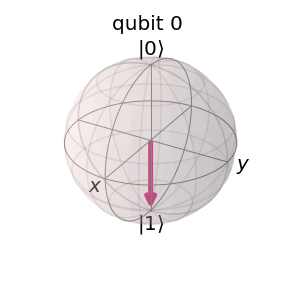
\includegraphics[scale = 0.75]{../Demonstration/img/Quantum_essentials_1.PNG}
\caption{A Bloch sphere representation of 1 qubit in the |1> state. The Bloch sphere clearly indicates that the state of a qubit has a certain probabilistic aspect to it.}
\end{figure}

\subsection{Superposition and entanglement}

\textbf{Superposition} is a term a lot of people have heard about and how it could achieve major breakthroughs in the scientific world, but what does it exactly represent is the real question. Quantum advantage is mostly gained from this quantum principle, where a quantum particle can remain in both states at once whilst it has not been observed. To explain this more clearly from a computer science angle, a qubit in superposition is during execution behaving as 0 and 1 at the same time. A concept that seems impossible within a classical frame of mind but also very advantageous if you know where to look. To put it more clearly, e.g. if you are processing a big array of data through your processor, your processor will take one item of the array, process, convert and output it before it will take another item of the array and perform the same thing. A quantum computer could go about this process in a similar yet much more ingenious way. A quantum processor would put an amount of qubits in superposition to represent the array as input, perform the needed amount of quantum gates and receive the output in a single go instead of needing to loop over the full array. ~\autocite{Draper2000}

\textbf{Entanglement} is another major principle within the realm of quantum physics. It refers to the correlation between entangled qubits where the state of one qubit influences the state of the correlated qubit in a way that it can be exploited theoretically infinitely speed up computation. This entanglement can be achieved inside a quantum computer by the use of quantum gates on qubits in a state of superposition. The deterministic result of the qubits at the end of an experiment will show the same correlation in the results, keeping in mind that enough experiments are performed to defend against quantum decoherence mistakes and other external influences.
~\autocite{fern2016mathematics}

These two principles are constantly being used  by a quantum processor as the one that Google showed of in their latest showcase of their quantum supremacy, ~\textcite{Google2019}. Together they are able to exponentially increase the computing power of a quantum computer, as you add more and more qubits you are exponentially increases the available data items such a processor could handle. For example to be able to simulate the biggest medicine of the 20th century, penicillin you would need 286 functional qubits, which in turn would be able to generate the $2^{286}$ bits of memory. This amount of memory is impossible to be able to achieved with a classical amount of bits, while a quantum computer in turn would be able to complete the simulations with theoretically 286 stable qubits. Actually getting to such a stable amount of qubits in itself will still be a scientific miracle. 





